\documentclass[a6paper,fontsize=10pt,twoside,openright]{scrbook}
\usepackage[a6paper,top=1cm,bottom=1.9cm,left=1cm,right=1cm,footskip=1cm,headsep=0.2cm]{geometry}
\usepackage[swedish]{babel}
\usepackage{graphicx,tocloft,metalogo,makeidx,titletoc,fontspec,titlesec,eso-pic,scrpage2,anyfontsize,lipsum,microtype}

%\usepackage{showframe}
\vbadness=10001
\makeindex

%% eso-pic for background on chapter pages %%
\newcommand\BackgroundPic{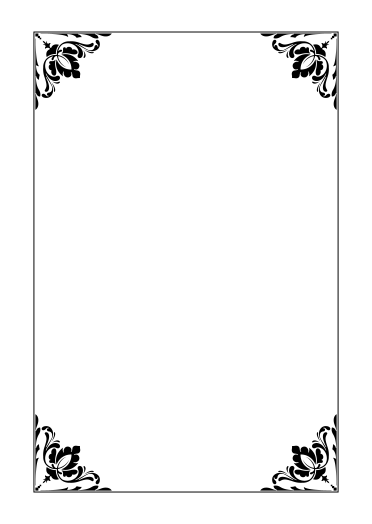
\includegraphics[width=\paperwidth,height=\paperheight,keepaspectratio]{chapter.pdf}}

%% scrpage2 pagestyling %%
\pagestyle{scrheadings}
\clearscrheadfoot

%% change empty page produced by \cleardoublepage into scrheading style %%
\makeatletter
\let\ps@empty\ps@scrheadings
\makeatother

%% chapter and section styling %%
\titleformat{\chapter}[hang]{}{}{0pt}{\centering\fontsize{40}{70}\selectfont\chapterfont}
\titleformat{\section}[hang]{}{}{0pt}{\textbf}
\titlespacing*{\section}{0pt}{10pt}{1pt}
\titlecontents{chapter}[0em]{\addvspace{3pt}}{\contentslabel{}}{}
              {\titlerule*[0.4pc]{.}\contentspage}
\newfontfamily\chapterfont[]{ChopinScript}

%% Command for chapter page, will remove foot and head %%
\newcommand{\chapterpage}[2]{
  \cleardoublepage
  \AddToShipoutPicture*{\BackgroundPic}
  \chapter[#1]{#2}
  \renewcommand{\leftmark}{#1}
  \newpage
  \ohead{\textsc{\scriptsize\leftmark}}
  \ofoot[\pagemark]{\scriptsize\pagemark}
  \cfoot{\centering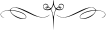
\includegraphics[keepaspectratio]{footelement.pdf}}
}
\makeatletter
\renewcommand\chapter{\if@openright\cleardoublepage\else\clearpage\fi
  \thispagestyle{empty}
  \global\@topnum\z@
  \@afterindentfalse
  \ofoot[\pagemark]{}
  \cfoot{}
  \ohead{}
  \secdef\@chapter\@schapter}
\makeatother

%% Command for songs %%
\newcommand{\visa}[2]{
  \index{#1}
  \index{#2}
  \section{#1}
}

%% TOC %%
\setcounter{tocdepth}{0}
\tocloftpagestyle{scrheadings}

%% MISC %%
\pagenumbering{arabic}
\renewcommand{\chaptername}{}
\renewcommand{\thechapter}{}
\renewcommand{\thesection}{}

\begin{document}
\vspace*{7cm}
\hspace*{1cm}
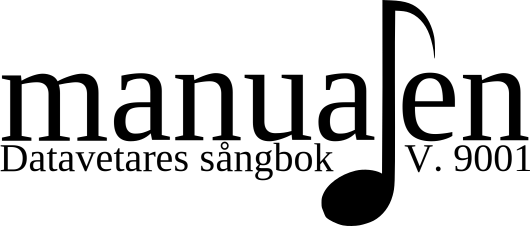
\includegraphics[keepaspectratio,width=7cm]{logo.pdf}
\clearpage
\noindent Denna manualen tillhör:
\ohead{\textsc{\scriptsize\leftmark}}
\ofoot[\pagemark]{\scriptsize\pagemark}
\clearpage
\null
\clearpage
\null
\vfill
    {\noindent\centering
      
      Logotyp: Jens Bohlin\\
      Producerad med \XeTeX\\
      Tryckår: 2014\\
      Tryckeri: ?\par
    }
\cleardoublepage
\cfoot{\centering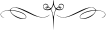
\includegraphics[keepaspectratio]{footelement.pdf}}
    {\noindent\large\textrm{\textbf{FÖRORD}}\vspace*{10pt}}\\
    \indent\lipsum[1-4]
%% begin toc on odd page and style the title %%
\cleardoublepage
\renewcommand{\contentsname}{\vspace{-2.1cm}\large\textrm{INNEHÅLL}\vspace{-1.2cm}}
\tableofcontents

%% Remove the toc title from heading %%
\renewcommand{\leftmark}{}

\chapterpage{Av tradition}{Av tradition}
%% \fancyhead[RO,LE]{\textsc{\scriptsize\leftmark}}

\section{DU GAMLA, DU FRIA}
Du gamla, Du fria, Du fjällhöga nord\\
Du tysta, Du glädjerika sköna!\\
Jag hälsar Dig, vänaste land uppå jord,\\
/: Din sol, Din himmel, Dina ängder gröna. :/\\
\\
Du tronar på minnen från fornstora dar,\\
då ärat Ditt namn flög över jorden.\\
Jag vet att Du är och Du blir vad du var.\\
/: Ja, jag vill leva jag vill dö i Norden. :/\\
\\
Jag städs vill dig tjäna mitt älskade land,\\
din trohet till döden vill jag svära.\\
Din rätt, skall jag värna, med håg och med hand,\\
/: din fana, högt den bragderika bära. :/\\
\\
Med Gud skall jag kämpa, för hem och för härd,\\
för Sverige, den kära fosterjorden.\\
Jag byter Dig ej, mot allt i en värld\\
/: Nej, jag vill leva jag vill dö i Norden. :/\\
\\
{\footnotesize\textit{
    Text: Richard Dybeck, 1844\\
    \\
    Sveriges nationalsång av tradition sedan 1866.\\
    De två sista verserna sjungs sällan.
}}
\clearpage
\section{SVERIGES FLAGGA}
Flamma stolt mot dunkla skyar\\
lik en glimt av sommarens sol!\\
Över Sveriges skogar, berg och byar,\\
över vatten och viol!\\
Du som sjunger, när Du bredes\\
som vår gamla lyckas tolk.\\
Solen lyser! Solen lyser!\\
Ingen vredes åska slog vårt tappra folk!\\
\\
Flamma högt vårt kärlekstecken!\\
Värm oss, när det blåser kallt!\\
Stråla ut de blåa vecken\\
kärlek mera stark än allt!\\
Sveriges flagga! Sveriges ära!\\
Fornklenod och framtidstolk!\\
Gud är med oss! Gud är med oss!\\
Han skall bära stark vårt fria svenska folk\\
\\
{\footnotesize\textit{
    Text: K.G. Ossiannilsson\\
    Musik: Hugo Alfvén
}}
\chapterpage{Datavetarvisor}{Datavetarvisor}
\visa{THE BASIC SONG}{10 LET oss nu fatta i våra glas}
{\footnotesize\textit{Melodi: Mors lilla Olle}}\\
\texttt{10 LET oss nu fatta i våra glas\\
  20 INPUT en klunk utav det som där has\\
  30 IF du fått nog THEN till 50 min vän\\
  40 ELSE GOTO-baka till 10 igen\\
  50 END\\
}
\\
{\footnotesize\textit{Inledande radnummer sjungs ej. I övrigt följs kommandon, ex drick vid "INPUT en klunk..."}}
\clearpage
\chapterpage{Snapsvisor}{Snapsvisor}
\chapterpage{Ölvisor}{Ölvisor}
\chapterpage{Vinvisor}{Vinvisor}
\chapterpage{Avecvisor}{Avecvisor}
\chapterpage{Gasquevisor}{Gasquevisor}
\chapterpage{Säsongsvisor}{Säsongsvisor}
\chapterpage{Visor på Svenska}{Visor på\\Svenska}
\chapterpage{Osvenska visor}{Osvenska visor}
\chapterpage{Register}{Register}
\backmatter
\renewcommand\indexname{}
\printindex
\end{document}
